\documentclass{beamer}

\usepackage{listings}
\usepackage{hyperref}
\usepackage{textpos}

\usecolortheme{crane}
\useoutertheme{infolines}
\usefonttheme[onlymath]{serif}

\title{HorseIR : An Array-based Approach to SQL Queries}
\author{Hongji Chen}
\date{August 30, 2017}

\begin{document}
\maketitle

\addtobeamertemplate{frametitle}{}{%
\begin{textblock*}{100mm}(.85\textwidth,-1cm)
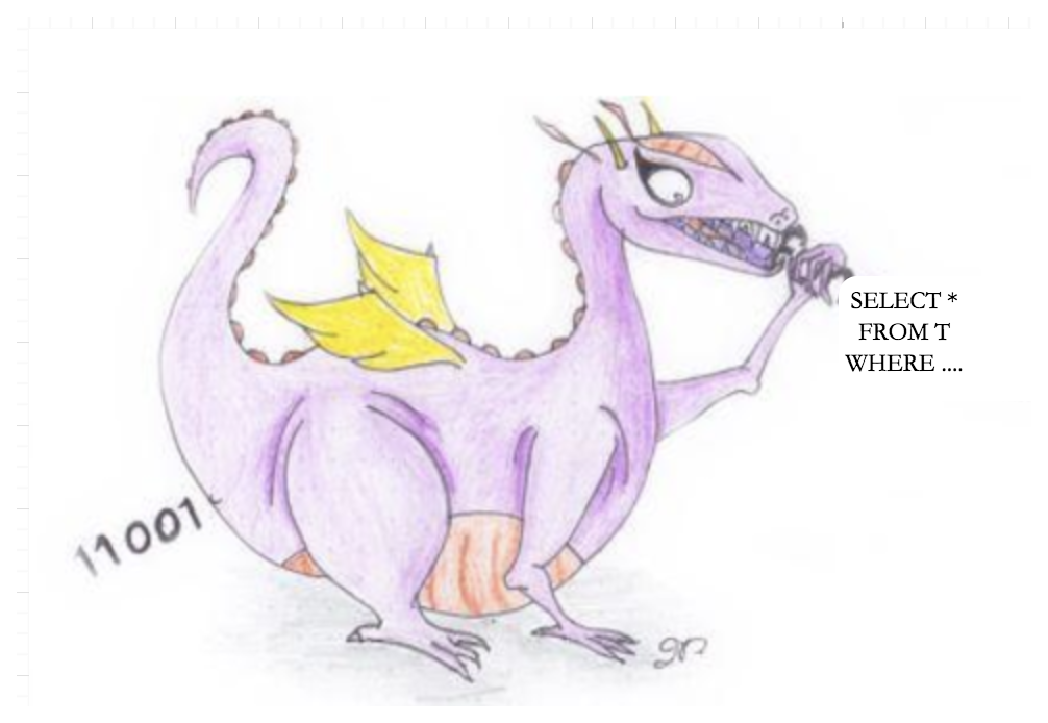
\includegraphics[width=1.5cm,keepaspectratio]{logo-dragon}
\end{textblock*}}

\begin{frame}{What is HorseIR?}
\begin{itemize}
    \item array-based programming language   
    \item uniform intermediate representation(IR) 
    \item optimization framework 
\end{itemize}
\vskip 0.5in
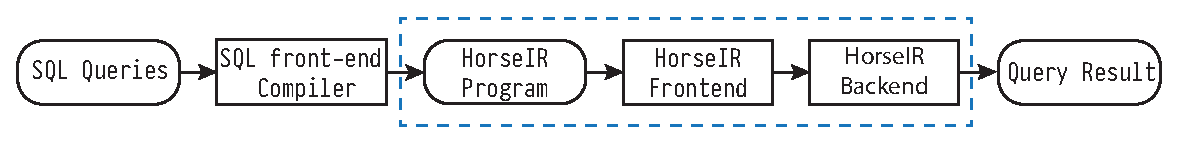
\includegraphics[width=\textwidth]{horse-flow}
\end{frame}

\begin{frame}{What is HorseIR?}
\centering
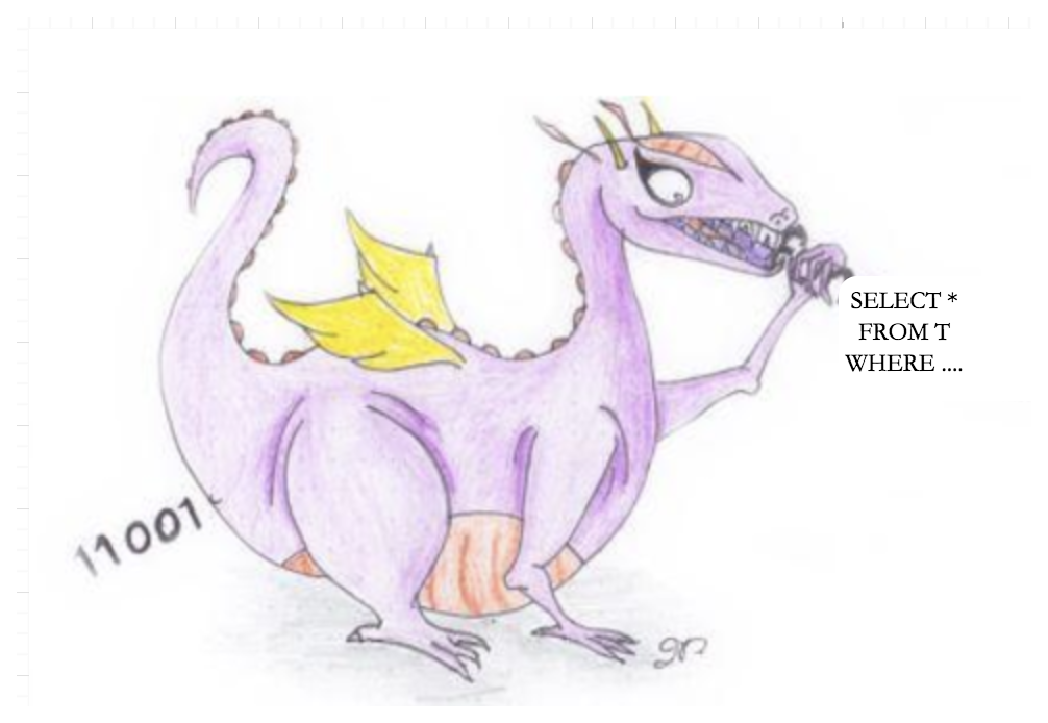
\includegraphics[width=\textwidth]{logo-dragon}
\end{frame}

\begin{frame}{In-memory Database System and \\ IR-based Query Engine}
\begin{itemize}
    \item row-oriented or column-oriented systems
          \begin{itemize}
          \item row-oriented storage: run as few operation as
                possible on row record (most database use-case, e.g. logging)
          \item column-oriented storage: good for set operations for whole
                table data (e.g. analytics)
          \end{itemize}
    \item complex primitives set or reduced primitives set
    \item user-defined functions (UDF) 
          \begin{itemize}
          \item not in SQL standard, but as a language extension in most
                systems
          \item flexibility?
          \item optimize potential?
          \end{itemize}
    \item parallel code generation
\end{itemize}
\end{frame}

\begin{frame}[fragile]{Related Work - In-memory Database Systems}
\begin{itemize}
\item SQLite
      \begin{itemize}
      \item \href{https://sqlite.org/opcode.html}
                 {https://sqlite.org/opcode.html}
      \end{itemize}
      \item MonetDB
      \begin{itemize}
      \item Stratos Idreos, Fabian Groffen, Niels Nes, Stefan Manegold,
            K. Sjoerd Mullender, and Martin L. Kersten. 2012. MonetDB:
            Two Decades of Research in Column-oriented Database
            Architectures. IEEE Data Eng. Bull. 35, 1 (2012), 40–45.
      \item \href{http://sites.computer.org/debull/A12mar/monetdb.pdf}
                 {http://sites.computer.org/debull/A12mar/monetdb.pdf}
      \end{itemize}
      \item KDB+ System
      \begin{itemize}
      \item \href{https://kx.com}{https://kx.com}
      \end{itemize}
\end{itemize}
\end{frame}

\begin{frame}{SQLite}
\begin{itemize}
\item SQLite Bytecode
      \begin{itemize}
      \item scalar based IR design
      \item dynamically typed
      \item no optimization on bytecode level
      \item designed for register based virtual machine
      \end{itemize}
\end{itemize}
\end{frame}

\begin{frame}[fragile]{MonetDB}
\begin{itemize}
    \item pioneer in IR based execution engine design
    \item MonetDB Assembly language(MAL)
          \begin{itemize}
          \item scalar based IR design
          \item statically strongly typed, without sub-typing 
          \item encapsulate atomic relational algebra operation in each
                instruction
          \item frontend translate queries into MAL
          \item backend interpret MAL to generate result
          \item optimizer optimize MAL to MAL
          \end{itemize}
\end{itemize}
\end{frame}

\begin{frame}{KDB+ System}
\begin{itemize}
    \item K and Q programming language
          \begin{itemize}
          \item fully functional programming (not IR-based)
          \item array-based language design (array/vector are first-class type)
          \item focus on data analytics
          \item powerful and efficient primitives implementation
          \item limited intra-procedural or inter-procedural optimization
          \end{itemize}
\end{itemize}
\end{frame}

\begin{frame}{Related Work Summary} 
\small {
\begin{table}[]
\label{my-label}
\begin{tabular}{l|lll}
Database System   & SQLite       & MonetDB           & KDB+ System           \\
\hline
Language Design   & scalar-based & scalar-based      & array-based           \\
Storage Structure & row-oriented & column-oriented   & column-oriented       \\
Primitives        & reduced      & complex           & reduced               \\
UDF Support       & external     & MAL, external     & native                \\
Parallel Code     & limited      & explicit declared & implicit (primitives)
\end{tabular}
\end{table}
}
\end{frame}


\begin{frame}{HorseIR - Summary}
\begin{itemize}
    \item syntax design
    \item type system
    \item fully functional interpreter connected to Hanfeng's backend
\end{itemize}
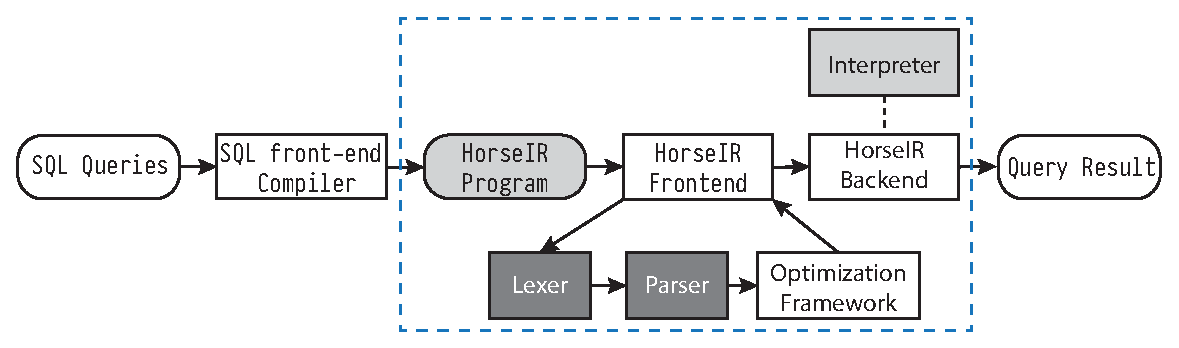
\includegraphics[width=\textwidth]{horse-finished}
\end{frame}

\begin{frame}{HorseIR}
\begin{itemize}
\item array-based IR design for database system
      \begin{itemize}
      \item reflects column-data storage in database system 
      \begin{itemize} 
      \item homogeneous data type storage 
      \item vector-based column
      \end{itemize}
      \item explore data parallelism easily 
      \begin{itemize}
      \item a rich set of array-based built-in functions
      \end{itemize}
      \item data compression friendly
      \end{itemize}
\item statically typed, with sub-typing
\end{itemize}
\end{frame}

\begin{frame}[fragile]{HorseIR - A Quick Example}
\begin{lstlisting}[language=SQL]
SELECT LastName FROM EmployeeTable;
\end{lstlisting}
\begin{lstlisting}[basicstyle=\small]
module default {
    import Builtin.*;
    def main() :table {
        t0   :table     = @load_table(`EmployeeTable) ;
        name :sym       = check_cast(
            @column_value(t0, `LastName), 
            sym
        ) ;
        t1   :list<sym> = @enlist(`LastName) ;
        t2   :list<sym> = @enlist(name) ;
        t3   :table     = @table(t1, t2) ;
        return t3 ;
    }
}
\end{lstlisting}
\end{frame}

\begin{frame}{HorseIR}
\begin{itemize}
    \item column-oriented system (use vector as a abstract view of column)
    \item reduced primitive set
          \begin{itemize}
          \item efficient implementation
          \item expose details to optimizer
          \end{itemize}
    \item UDF implementation:
          \begin{itemize}
          \item write UDF in arbitrary language
          \item compile into HorseIR
          \item participate in optimization
          \end{itemize}
    \item parallel code generation:
          \begin{itemize}
          \item at primitive level
          \item at intra-procedural level
          \item at inter-procedural level
          \end{itemize}
\end{itemize}
\end{frame}

\begin{frame}[fragile]{HorseIR}
\begin{lstlisting}[language=SQL, basicstyle=\small]
CREATE TABLE Employee 
(LastName varchar(99), DepartmentID int);
CREATE TABLE Department 
(DepartmentID int, DepartmentName varchar(99));

select * from Employee,Department
where Employee.DepartmentID = Department.DepartmentID;
\end{lstlisting}
\end{frame}

\begin{frame}{Types in HorseIR}
\begin{itemize}
    \item designed for database systems
          \begin{itemize}
          \item string and character
          \item numerics (integer and floating-point)
          \item date and time
          \item functions
          \item table and keyed table
          \end{itemize}
    \item parametric polymorphism
          \begin{itemize}
          \item list (list<?>)
          \item dictionary (dict<?, ?>)
          \item enumeration (enum<?>)
          \end{itemize}
\end{itemize}
\end{frame}

\begin{frame}[fragile]{Types in HorseIR}
\begin{itemize}
    \item statically checked and inferred at compile time
    \item resolve overloading and polymorphic dispatch at compile time
          \begin{itemize}
          \item minimize runtime overhead
          \end{itemize}
    \item downcast guard elimination
          \begin{lstlisting}
x :?
castedX :i32 = check_cast(x, i32); (*)
avgX :i32 = @Builtin.avg(castedX);    
          \end{lstlisting}
          Is it possible to safely remove this cast? use static analysis
\end{itemize}
\end{frame}

\begin{frame}[fragile]{Types in HorseIR - Overloading}
\begin{itemize}
    \item support more flexible UDF
    \item choose the most efficient primitive implementation at compile time
          \begin{itemize}
          \item function overloading
          \end{itemize}
\end{itemize}

\begin{lstlisting}
def foo(x: ?, y :?) :bool {
    avgX :? = @Builtin.avg(x) ; 
    result :bool = @Builtin.lt(y, avgX);
    return result;
}
@Builtin.avg(?) @Builtin.avg(f64) @Builtin.avg(i32) 
\end{lstlisting}
\begin{itemize}
    \item choose which implementation?
          \begin{itemize}
               \item in foo(i32, i32),
               \item in foo(f64, i32),
               \item in foo(list<i32>, i32)
          \end{itemize}
\end{itemize}
\end{frame}

\begin{frame}{HorseIR Frontend}
\begin{itemize}
    \item a lexer and parser
    \item interpreter
    \item customized abstract syntax tree
    \item optimization framework
          \begin{itemize}
          \item peephole
          \item static analysis
          \end{itemize}
\end{itemize}
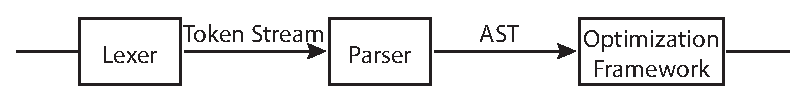
\includegraphics[width=\textwidth]{horse-frontend}
\end{frame}

\begin{frame}{Conclusion}
\begin{itemize}
    \item HorseIR
          \begin{itemize}
          \item array-based IR for database system with powerful primitives
          \item programming language optimizations for databases
          \item extensible framework for user-defined functions (UDF)
          \item efficient parallel code generation
          \end{itemize}
          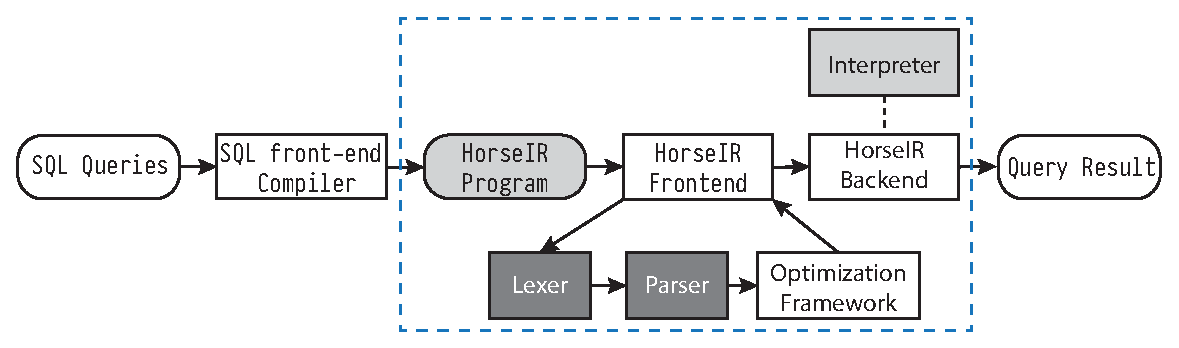
\includegraphics[width=0.9\textwidth]{horse-finished}
    \item complete working system
    \item future experiment on TPC-H benchmarks
\end{itemize}
\end{frame}

\begin{frame}{Questions?}
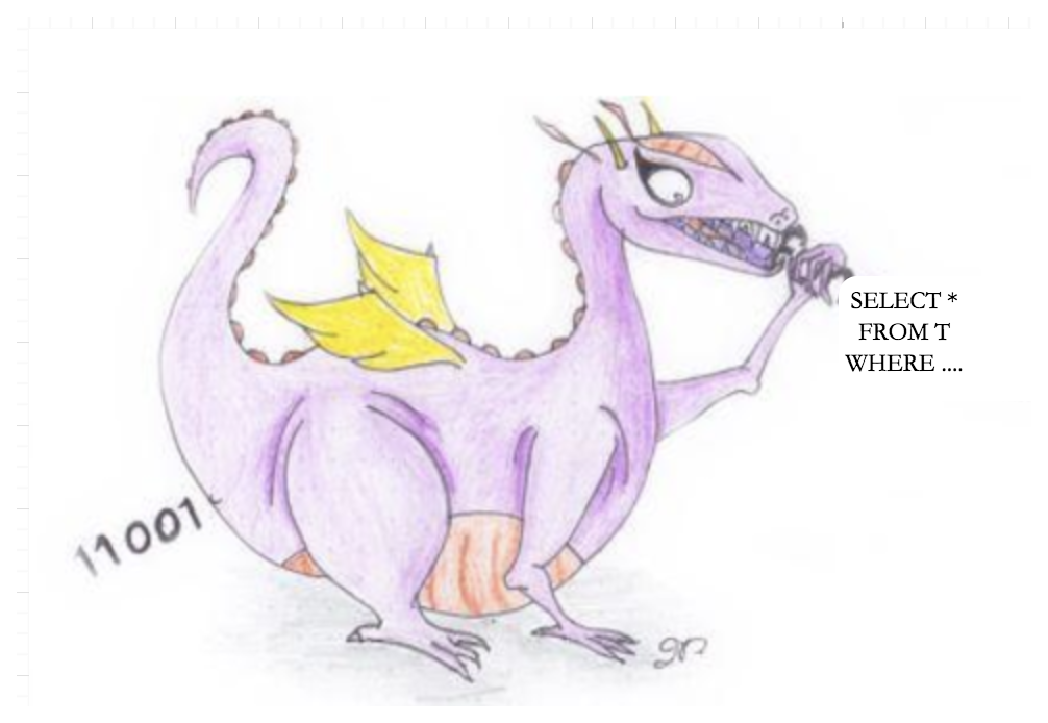
\includegraphics[width=\textwidth]{logo-dragon}
\end{frame}

\end{document}